%\documentclass[notes,10pt,aspectratio=169]{beamer}

%\documentclass[notes, 10pt,aspectratio=169]{beamer}
\documentclass[10pt,aspectratio=169]{beamer}


% Add this line to your preamble
%\setbeameroption{show notes on second screen=right}

%\usetheme{Singapore} %Boadilla, Madrid, default, etc. 
\usetheme[progressbar=frametitle]{metropolis}
\usecolortheme{rose} %beaver, dolphin, crane, 


\setbeamersize{text margin left=4mm, text margin right=4mm}


\usecolortheme{default}

\usepackage[utf8]{inputenc}
\usepackage[T1]{fontenc}
\usepackage{lmodern}
\usepackage{xcolor}
\usepackage{tikz}
\usepackage{booktabs} % Required for \toprule, \midrule, \bottomrule
\usetikzlibrary{shapes.geometric, arrows, positioning}

\tikzstyle{block} = [rectangle, draw, text width=4cm, align=center, rounded corners, minimum height=1cm]
\tikzstyle{decision} = [rectangle, draw, text width=5cm, align=center, fill=blue!10, rounded corners, minimum height=1cm]
\tikzstyle{terminal} = [rectangle, draw, text width=4.5cm, align=center, fill=yellow!30, rounded corners, minimum height=1cm]
\tikzstyle{end} = [rectangle, draw, text width=5cm, align=center, fill=green!30, rounded corners, minimum height=1cm]
\tikzstyle{arrow} = [->, thick]



\usepackage{adjustbox}
%2. change the bullets 
\setbeamertemplate{itemize item}[triangle] %circle, square,... 


% 1. Define custom colors and set colors 
%\definecolor{myblue}{HTML}{003366}
\definecolor{accent}{RGB}{78,205,196}

%\setbeamercolor{title}{fg=white,bg=myblue}
\setbeamercolor{frametitle}{fg=black,bg=white}
%\setbeamercolor{normal text}{fg=mygray}
\setbeamercolor{block title}{fg=black,bg=blue}
%\setbeamercolor{block body}{fg=black,bg=white}

\setbeamercolor{item}{fg= orange!80} % Change bullet color
\setbeamercolor{button}{bg=orange, fg=white}



\AtBeginSection[]
{
  \begin{frame}{Outline}
    \tableofcontents[currentsection]%,hideothersubsections]
  \end{frame}
}

% 3. BibLaTeX settings
\usepackage[
  backend=biber,
  style=apa,
  citestyle=authoryear
]{biblatex}
\addbibresource{../references.bib}

\title{Equilibrium effects of price updating: evidence from a centralized marketplace for annuities}
%\subtitle{A Mini Literature Overview}

\author{%
 Lucas Condeza
\inst{1} \and
   %\and
%  Coauthor Three\inst{3}
}
\institute{
  \inst{1} Yale University \\
}

\date{\today}

\begin{document}

\begin{frame}
  \titlepage
\end{frame}



 %%%%%%%%% Slide 2  %%%%%%%%%%%%%

\begin{frame}{Motivation}\label{slide:motivation}
\begin{itemize}
    \item  In several markets consumers receive initial offers, then they can request revised offers. Examples: 
    \begin{itemize}
        \item Loans: consumers get a loan estimate (LE) and showing a LE to another lender could lead to a revised offer. \hyperlink{slide:fig_LE}{\beamerbutton{Loan Estimate}} %[\href{https://chatgpt.com/share/68eaf593-1518-800d-b874-1fba1adbe177}{1}]
        \item Auto dealerships: buyers can shop around and dealers are willing to revise their initial offers %[\href{https://chatgpt.com/share/68eaf593-1518-800d-b874-1fba1adbe177}{2}]
    \end{itemize}

    \item What is  the welfare impact of allowing consumers to request revised offers?
    \item Effects of prohibiting revised offers: 
    
    \begin{itemize}
        \item Direct impact: buyer can no longer improve initial offer. 
        \item Indirect effect: buyers improve their initial offers 
    \end{itemize}

    %Economic forces at play: 
    %\begin{itemize}
    %    \item Learning: firms learn competitors' prices and can best respond.
    %  \item Discrimination: if search cost are correlated with preferences. [not today] 
    %\end{itemize}
    \note{Mention that only firms who made an initial offer can revise their offers. }
    
\end{itemize}

\note{
    \begin{itemize}
        \item I am going to study the effects of being able to request revised offers in a centralized marketplace for annuities in Chile.  
    \end{itemize}}


\end{frame}

%%%%%%%%% Slide 3 %%%%%%%%%%%%%

\begin{frame}{This research}
\begin{itemize}
    \item Studies a centralized marketplace for annuities in Chile (SCOMP)
    \item A recent law eliminated the possibility of requesting revised offers.
    \begin{itemize}
        \item Before: consumers receive initial offers, then can request revised offers from one firm.
        \item After: consumers can only accept/reject initial offers.
        \item Rationale for elimination: "firms will not make their best efforts in the initial phase"
    \end{itemize}
    %\item Also provides evidence on asymmetries in information precision in selection markets. 
\end{itemize}
\end{frame}

 %%%%%%%%% Slide 4 %%%%%%%%%%%%%
\begin{frame}{Literature}
\begin{itemize}
    \item Search in selection markets: \textcite{allen_search_2019} %larsen_efficiency_2021

    \item Competition in selection markets: \textcite{mahoney_imperfect_2017, crawford_asymmetric_2018,
    cuesta_price_2018, cosconati_competing_2025} 

    \item Centralized marketplaces in selection markets : \textcite{abaluck_when_2023,tebaldi_estimating_2025} 
    
    \item SCOMP specific: \textcite{boehm_intermediation_2024, illanes_retirement_2019, alcalde_intermediary_2021}
    
    %\item Selection in multiple dimensions: \textcite{finkelstein_adverse_2004} and Finkelstein and McGarry (2006).  

    %\item Aftermarkets: \textcite{allen_search_2019} %larsen_efficiency_2021   
\end{itemize}
\note{
\textcolor{blue}{ ADD THE CONTRIBUTIONS TO EACH LITERATURE AND ADD MORE PAPERS}
}
\end{frame}

%%%%%%%%%

\section{Setting and Data}

%%%%%%%%% Slide 6 %%%%%%%%%%%%%
\begin{frame}{Setting: annuities}\label{slide:setting}
    
    \begin{itemize}%[<+->]
    \item Annuities: transform a stock of savings into a stream of payments until death.
    \item Reasons to buy: insure against overlife risk
        \item Profits of firm $j$: 
    \begin{align*}
    \pi_{ji}(F) = S_i-  \mathbb{E}^j_{T} \left[\sum_{t=1}^T\frac{F}{(1+r_j)^t}|x_i \right]
    \end{align*}
    % if it was only financing cost, it would be a monopoly
   
     $S$: stock of savings, $F$: per period annuity payment, $x_i$: buyer mortality factors
    
    \item Firm heterogeneity: algorithm (mortality tables), financing costs ($r_j$) and risk ratings. 
    
    \end{itemize}


    \note{
    \begin{itemize}
        \item Explicitly not link the annuities market with pensions because generates confusion
        \item Explain what annuities are. 
        \item Mention that $x_i$ is not firm specific. Firms observe the same covariates.
        \item Explain that the risk rating is a measure of the bankruptcy risk of the firm, I am assuming that only affects demand.
    \end{itemize}}
\end{frame}

%%%%%%%%% Slide 7 %%%%%%%%%%%%%
\begin{frame}{SCOMP Process}\label{slide:setting2}
\begin{center}
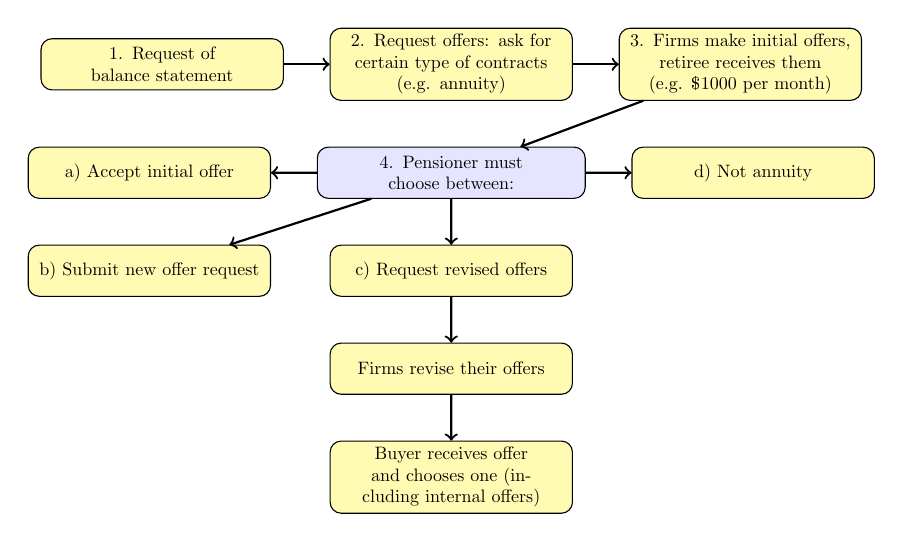
\begin{tikzpicture}[node distance=.9cm and .9cm, scale=0.65, every node/.style={transform shape}]

\node[terminal] (step1) {1. Request of \\  balance statement};
\node[terminal, right=of step1] (step2) {2. Request offers: ask for certain type of contracts \\ (e.g. annuity) };
\node[terminal, right =of step2] (step3) {3. Firms make initial offers, \\ retiree receives them (e.g. \$1000 per month)};

% **CHANGES MARKED**: Second row - right to left
\node[decision, below=of step2] (step4) {4. Pensioner must\\choose between:};



% 2. Place the outcome nodes relative to the central node
\node[terminal, left = of step4] (choice_a) {a) Accept initial offer};
\node[terminal, below left = of step4] (choice_b) {b) Submit new offer request}; % Position relative to choice_a
\node[terminal, right= of step4] (choice_d) {d) Not annuity};
\node[terminal, below =of step4] (choice_c) {c) Request revised offers}; % Position relative to choice_d









% Additional choices below decision
\node[terminal, below=of choice_c] (choice_c2) {Firms revise their offers};
\node[terminal, below=of choice_c2] (choice_c3) {Buyer receives offer and chooses one (including internal offers)};


% **CHANGES MARKED**: Third row - decision and outcomes (left to right)
%\node[terminal, left =of step4] (choice_a) {a) Accept\\initial offer};
%\node[terminal, below= of step4 ] (choice_b) {b) Submit new\\offer request};
%\node[terminal, below =1.2cm of step4] (choice_c) {c) Request\\revised offers};
%\node[terminal, right =1.2cm of step4] (choice_d) {d) Not annuity};


% **CHANGES MARKED**: Horizontal flow arrows - first row (left to right)
\draw[arrow] (step1) -- (step2);
\draw[arrow] (step2) -- (step3);
\draw[arrow] (step3) -- (step4);

% **CHANGES MARKED**: Second row arrows (right to left)
%\draw[arrow] (choice_b) -- (choice_b2);
\draw[arrow] (step4) -- (choice_a);
\draw[arrow] (step4) -- (choice_b);
\draw[arrow] (step4) -- (choice_c);
\draw[arrow] (step4) -- (choice_d);


\draw[arrow] (choice_c) -- (choice_c2);
\draw[arrow] (choice_c2) -- (choice_c3);


\end{tikzpicture}
\end{center}
\begin{itemize}
    \item \hyperlink{slide:fig_offer_certificate}{\beamerbutton{Offer Certificate}}
\end{itemize}
\note{
Explain that: 
\begin{itemize}
    \item Mention that revise  offers are less regulated
    \item An exception to less regulation is that they can not be lower than initial offers. 
    \item only initial bidders can make revised offers 
    \item We do not observe requests only the revised offers. 
    \item When requesting revised offers, firms learn competitors' initial offers.
\end{itemize}
}
\end{frame}

%%%%%%%%% Slide 8 
\begin{frame}{Data} \label{slide:data}
\begin{itemize}
    \item SCOMP data at the individual level  
    \begin{itemize}
        \item Posted and revised offers, consumer acceptance. \textbf{Not} requests 
        \item Total savings 
        \item Demographics: age and gender \hyperlink{slide:fig_offer_certificate}{\beamerbutton{Certificate with initial offers}}
    \end{itemize}
     \item Retirement insurance companies: risk ratings
\end{itemize}

Particularities of the data/setting: 
\begin{itemize}
    \item One observes all the offers received by the buyers 
    \item One observes the same information as the firms (gender, age, savings)
\end{itemize}
\textcolor{red}{[best way of leveraging this particularities?]}
\note{
    \begin{itemize}
        \item I observe only the revised offers made not the requested ones. 

    \end{itemize}
}
\end{frame}



%%%%%%%%%%%%%%%%%%%%%%%%%%%%%%%%%%%%%%%%%%%%%%%%%%%%%%

\section{Empirical Evidence}
 
%%%%%%%%% Slide 10
\begin{frame}{Descriptive Evidence}\label{slide:Descriptive_evidence}

\begin{enumerate}
    \item Most buyers request revised offers and the improvement is sizeable. \hyperlink{slide:fig1}{\beamerbutton{Revised offers}} 
    \item Products are differentiated \hyperlink{slide:fig2}{\beamerbutton{Foregone value}} 
    \item Selection into companies \hyperlink{slide:fig3}{\beamerbutton{Heterogeneity in algorithm precision}}
    \item Firms learn about other firms' prices  \hyperlink{slide:fig4}{\beamerbutton{Learning}} 
\end{enumerate}
\end{frame}

%%%%%%%%% Slide 11
\begin{frame}\frametitle{Prevalence of revisions}\label{slide:fig1}
\begin{figure}
    \centering
    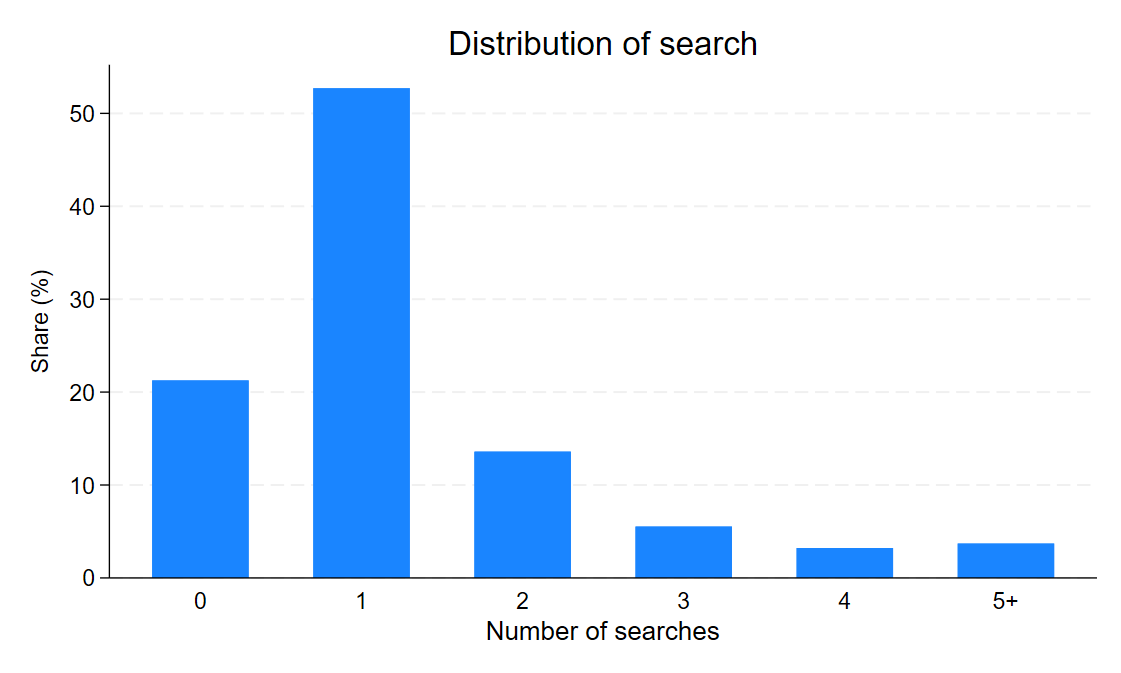
\includegraphics[width=0.49\textwidth]{../figures/IE3/IE3_dist_external_offers.png}
    \hfill 
    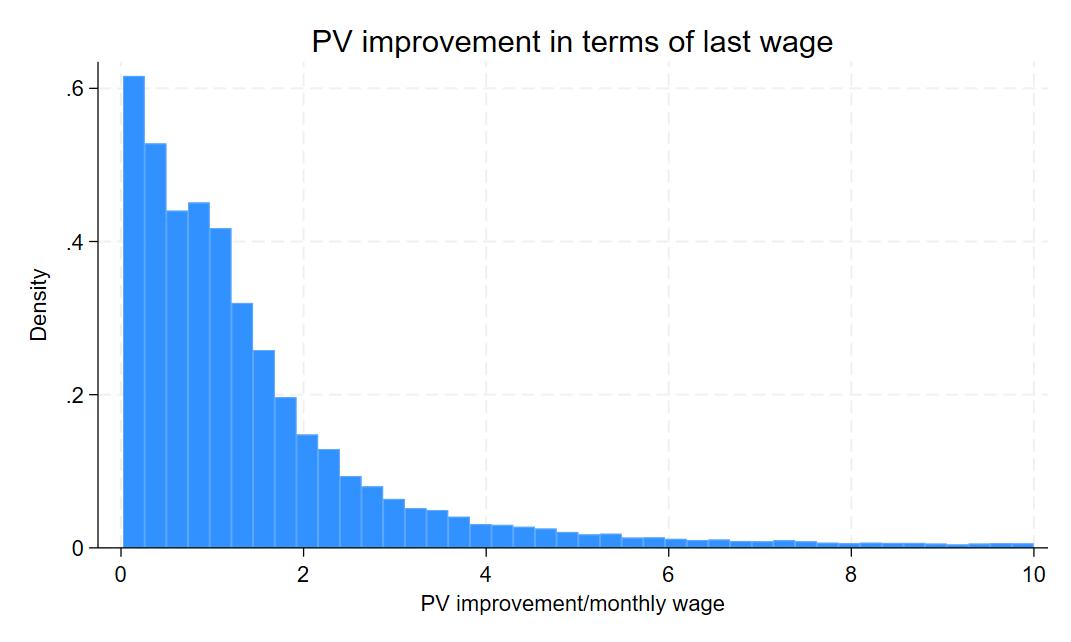
\includegraphics[width=0.49\textwidth]{../figures/IE3/IE3_offer_improvement_histogram.png}
\end{figure}

\begin{itemize}
    \item   75\% of the purchases are through revised offers. 
     \hyperlink{slide:Descriptive_evidence}{\beamerbutton{Go back}}   
    \item Not everyone requests revised offers $\rightarrow$ search costs. 
\end{itemize}

\note{
That only some people request revised offers suggests: 
\begin{itemize}
    \item There are search costs 
    \item Firms could be discriminating based on the search likelihood. 
\end{itemize}
Any assessment of the welfare effects of the aftermarket has to consider that by banning it buyers will save in search costs, but will not be able to improve on the initial posted prices. 

In a model where search costs are not correlated with valuations, the aftermarket prices by the sellers are the same as the initial prices.
}
\end{frame}

%%%%%%%%% Slide 12 %%%%%%%%%%%%%
\begin{frame}{Differentiation}\label{slide:fig2}    
Buyers do not always buy highest annuity. Average foregone value is 1.57 monthly wages.
\begin{figure}[H]
%\caption{}
\centering{}%
\begin{tabular}{cc}
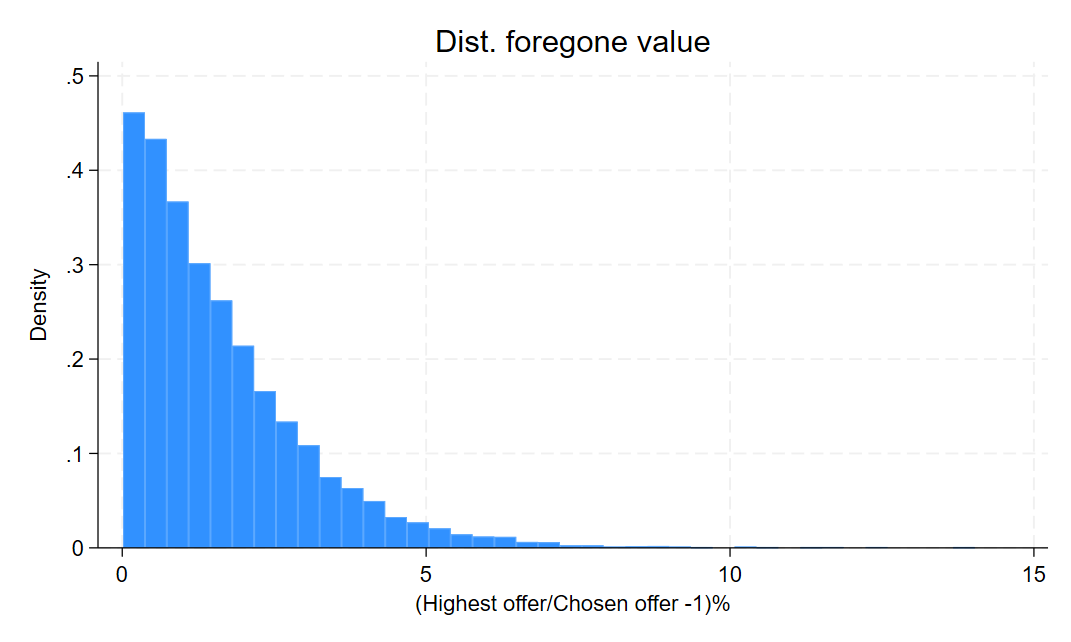
\includegraphics[scale=0.25]{../figures/IE3/IE3_foregone_hist.png}
\end{tabular}
\end{figure}
\hyperlink{slide:Descriptive_evidence}{\beamerbutton{Go back}}
\end{frame}


\begin{frame}{Algorithm precision} 
    \begin{itemize}
        \item If firms have different algorithms precision, e.g. the real type is $\theta_i$ and firm $j$ observes a signal $\hat{\theta}_{ij} \sim N(\theta_i, \sigma_j^2)$  

        \item [Work on this slide ]
    \end{itemize}
\end{frame}


%%%%%%%%%%%%%%%%%%%%%%%%%%%


\begin{frame}{Heterogeneity in algorithm precision}\label{slide:fig3}    
\begin{figure}[H]
%\caption{}
\centering{}%
\begin{tabular}{cc}
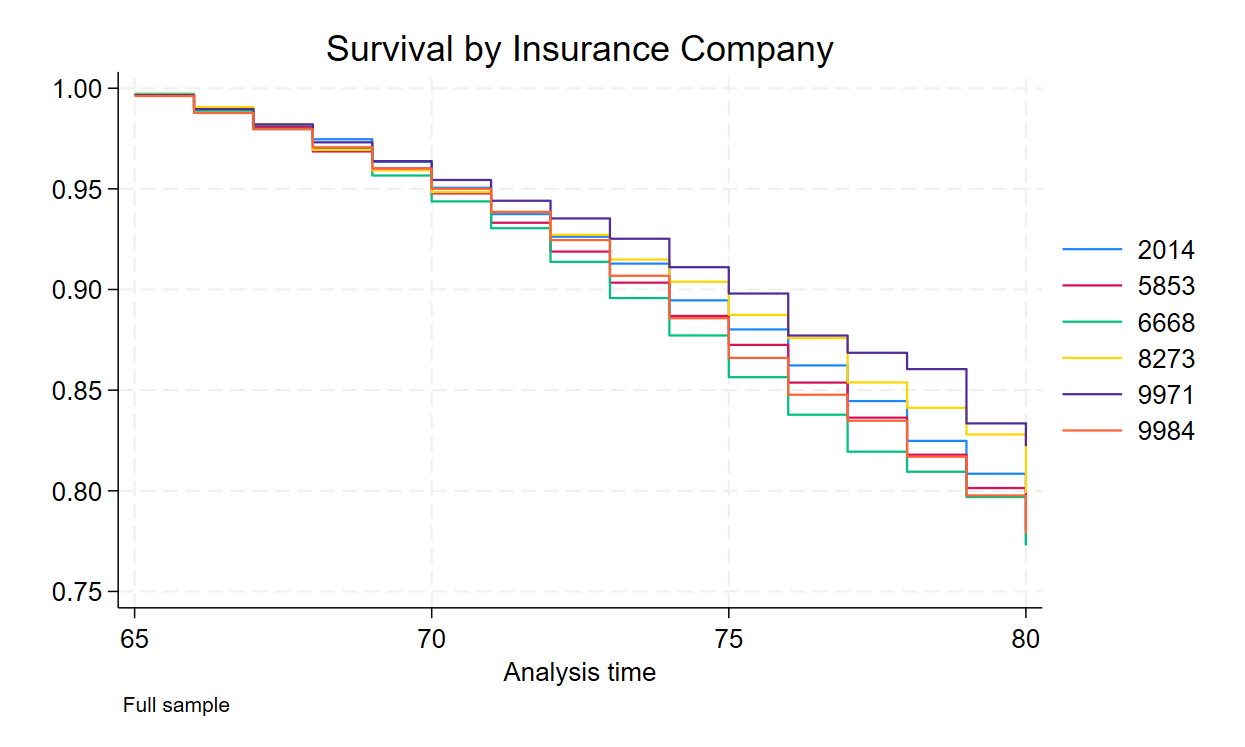
\includegraphics[scale=0.2964]{../figures/IE6/IE6_survival_year_all.png}
\end{tabular}
\end{figure}
\hyperlink{slide:Descriptive_evidence}{\beamerbutton{Go back}}
\end{frame}

%%%%%%%%% Slide 14 

\begin{frame}{Learning} 
    If firms do not know competitors' prices one expects them to increase their offers more when the competitors' prices are higher. 
    \begin{itemize}
        \item $$ F_{ij}^R - F_{ij}^I = \beta_0 + \beta_1 \text{Avg. gap}_{ij} + \beta_2 \text{Max. gap}_{ij} + \epsilon_{ij}$$

        \item $$ 1(F_{ij}^R  - F_{ij}^I)  = \alpha_0 + \alpha_1 \text{Avg. gap}_{ij} + \alpha_2 \text{Max. gap}_{ij} + \epsilon_{ij}$$
    \end{itemize}
    where  $$ \text{Avg. gap }_{ij} = \left(\frac{1}{J-1}\sum_{k \neq j} F_{ik}^I - F_{ij}^I\right) \quad \text{Max. gap } = \left(\max_{k \neq j} F_{ik}^I - F_{ij}^I\right)$$
    
\end{frame}


%%%%%%%%% Slide 15
\begin{frame}{Learning(1)}\label{slide:fig4}    
\scalebox{0.8}{
    {
\def\sym#1{\ifmmode^{#1}\else\(^{#1}\)\fi}
\begin{tabular}{l*{7}{c}}
\hline\hline
                    &\multicolumn{1}{c}{(1)}&\multicolumn{1}{c}{(2)}&\multicolumn{1}{c}{(3)}&\multicolumn{1}{c}{(4)}&\multicolumn{1}{c}{(5)}&\multicolumn{1}{c}{(6)}&\multicolumn{1}{c}{(7)}\\
                    &\multicolumn{1}{c}{Increase}&\multicolumn{1}{c}{Increase}&\multicolumn{1}{c}{Increase}&\multicolumn{1}{c}{Increase}&\multicolumn{1}{c}{Increase}&\multicolumn{1}{c}{Increase}&\multicolumn{1}{c}{Has External Offer}\\
\hline
main                &                     &                     &                     &                     &                     &                     &                     \\
Avg. Gap            &       0.316\sym{***}&       0.155\sym{***}&       0.155\sym{***}&       0.139\sym{***}&       0.147\sym{***}&       0.071\sym{***}&                     \\
                    &     (0.006)         &     (0.010)         &     (0.010)         &     (0.016)         &     (0.019)         &     (0.020)         &                     \\
[1em]
Max. Gap            &                     &       0.110\sym{***}&       0.110\sym{***}&                     &      -0.021         &      -0.006         &                     \\
                    &                     &     (0.009)         &     (0.009)         &                     &     (0.029)         &     (0.028)         &                     \\
[1em]
gap\_from\_avg        &                     &                     &                     &                     &                     &                     &      -0.191\sym{***}\\
                    &                     &                     &                     &                     &                     &                     &     (0.032)         \\
[1em]
Constant            &       1.893\sym{***}&       1.375\sym{***}&       1.375\sym{***}&       1.381\sym{***}&       1.387\sym{***}&       1.511\sym{***}&      -2.012\sym{***}\\
                    &     (0.010)         &     (0.082)         &     (0.082)         &     (0.045)         &     (0.046)         &     (0.121)         &     (0.028)         \\
\hline
Observations        &       14133         &       14133         &       14133         &        2046         &        2046         &        2046         &       16164         \\
\hline\hline
\multicolumn{8}{l}{\footnotesize Average: is the difference between the mean of other firms' initial offers and own initial offer}\\
\multicolumn{8}{l}{\footnotesize Max Gap: is the difference between the highest other firm's initial offer and own initial offer.}\\
\multicolumn{8}{l}{\footnotesize Cols (1)-(3) use the population of initial offers that are not the highest, (4)-(6) only use the highest offer}\\
\multicolumn{8}{l}{\footnotesize Cols (4) and (6) include firm fixed effects}\\
\end{tabular}
}

}

\hyperlink{slide:Descriptive_evidence}{\beamerbutton{Go back}}
\end{frame}

%%%%%%%%% Slide 16
\begin{frame}{Learning(2)}\label{slide:fig5}
  \begin{figure}[H]
%\caption{}
\centering{}%
\begin{tabular}{cc}
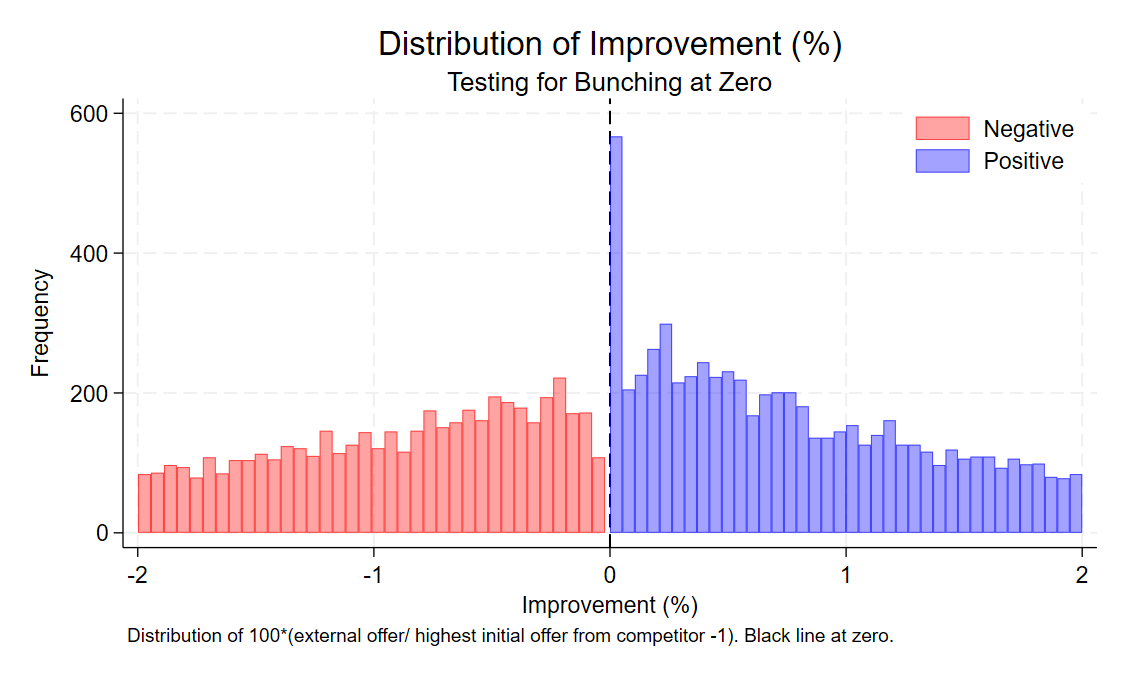
\includegraphics[scale=0.35]{../figures/IE7/IE7_hist_bunching_max(2).png} 
\end{tabular}
\end{figure}
\hyperlink{slide:Descriptive_evidence}{\beamerbutton{Go back}}
\end{frame}




%%%%%%%%%%%%%%%%%%%%%%%%%%%%%%%%%%%%%%%%%%%%%%%%%%%%%%%%%%%%%%%%%%%%%%%%%%%%%%%%
\section{Model and Simulations}

%%%%%%%%% Slide 17 %%%%%%%%%%%%% 

\begin{frame}{Learning Model: Overview}
\begin{itemize}
    \item \textbf{Goal:} Rationalize the increase in offers between initial and revised offers
    
    \item \textbf{Key mechanism:} Firms learn competitors' offers when consumer requests revised offers
    


    \item \textbf{Incorporate:}
    \begin{itemize}
        \item Search cost [not today]
        \item Product Differentiation [today]
        \item Prediction precision [not today]
        \item Learning [today]
    \end{itemize}

\end{itemize}
\end{frame}

%%%%%

\begin{frame}{Two-Stage Game: Timeline}\label{slide:timeline}
\begin{enumerate}
    \item \textbf{Stage 1 (Initial offers):} \hyperlink{slide:connection}{\beamerbutton{Connection with setting}}

    \begin{itemize}
        \item Firms draw costs $c_j$ from distribution $F(c_j|c_{-j})$ they only observe their own cost.
        \item Firms simultaneously post initial prices $p^{T1}_j$
        \item Consumer observes all offers
    \end{itemize}
    
    \vspace{0.3cm}
    
    \item \textbf{Consumer decision:}
    \begin{itemize}
        \item With probability $1-\lambda$: accepts one of the initial offers
        \item With probability $\lambda$: requests a revised offer from a randomly chosen firms
    \end{itemize}
    
    \vspace{0.3cm}
    
    \item \textbf{Stage 2 (Revised offers):}
    \begin{itemize}
        \item Selected firm observes all initial offers $p^{T1}$
        \item Can update its offer: $p^{T2}_j(c_j, p^{T1}) = \min(p^{T1}_j, p^*)$
        \item Consumer chooses among all available offers
    \end{itemize}
\end{enumerate}
\end{frame}

%%%%%

\begin{frame}{Second Stage: Optimal Pricing with Learning}
\textbf{When selected for revised offer, firm observes competitors' initial prices}

\vspace{0.3cm}

\textbf{Optimal updated offer:}
$$p^{T2}_j(c_j, p^{T1}) = \min(p^{T1}_j, p^*)$$

where
$$p^* = \arg\max_{p_j} (p_j - c_j) D_j(p_j, p^{T1}_{-j})$$

\vspace{0.3cm}
After observing competitors, firm best-responds to known prices rather than expected prices
\end{frame}

%%%%%

\begin{frame}{Expected Profits in Second Stage}
\textbf{When consumer searches, firm $j$ faces two scenarios:}

\vspace{0.3cm}

\textbf{1. Selected for revised offer ($\frac{1}{J}$ probability):}
$$\pi^{(j)}_j(p^{T1}, c_j) = (p^{T2}_j(c_j, p^{T1}) - c_j) D_j(p^{T2}_j(c_j, p^{T1}), p^{T1}_{-j})$$

\vspace{0.3cm}

\textbf{2. Competitor $j'$ selected ($\frac{1}{J}$ probability):}
$$\pi^{(j')}_j(p^{T1}, c_j, c_{j'}) = (p^{T1}_j - c_j) D_j(p^{T1}_{-j'}, p^{T2}_{j'}(c_{j'}, p^{T1}))$$

\vspace{0.5cm}

\textbf{Expected second stage profits:}
$$\pi^{T2}_j(p^{T1}, c_j, c_{-j}) = \frac{1}{J}\left[\pi^{(j)}_j(p^{T1}, c_j) + \sum_{j' \neq j} \pi^{(j')}_j(p^{T1}, c_j, c_{j'})\right]$$
\end{frame}

%%%%%

\begin{frame}{First Stage: Strategic Pricing}
\textbf{Firms anticipate the second stage when setting initial prices}

\vspace{0.5cm}

\textbf{Expected profits in first stage:}
$$\pi^{T1}_j(p^{T1}, c_j, c_{-j}) = (1-\lambda)\underbrace{(p^{T1}_j - c_j)D_j(p^{T1})}_{\text{Immediate acceptance}} + \lambda \underbrace{\pi^{T2}_j(p^{T1}, c_j, c_{-j})}_{\text{Search occurs}}$$

\vspace{0.5cm}

\textbf{Equilibrium condition:}
$$p^{T1}_j(c_j) = \arg\max_{p_j} \int \pi^{T1}_j(p_j, p^{T1}_{-j}(c_{-j}), c_j) dF(c_{-j}|c_j)$$

\vspace{0.3cm}
Trade-off: higher initial price (if accepted) vs. competitive position if search occurs

\textcolor{red}{How to compute equilibrium?}
\end{frame}


\begin{frame}{Simulations }
\begin{figure}[H]
\centering{}%
\begin{tabular}{cc}
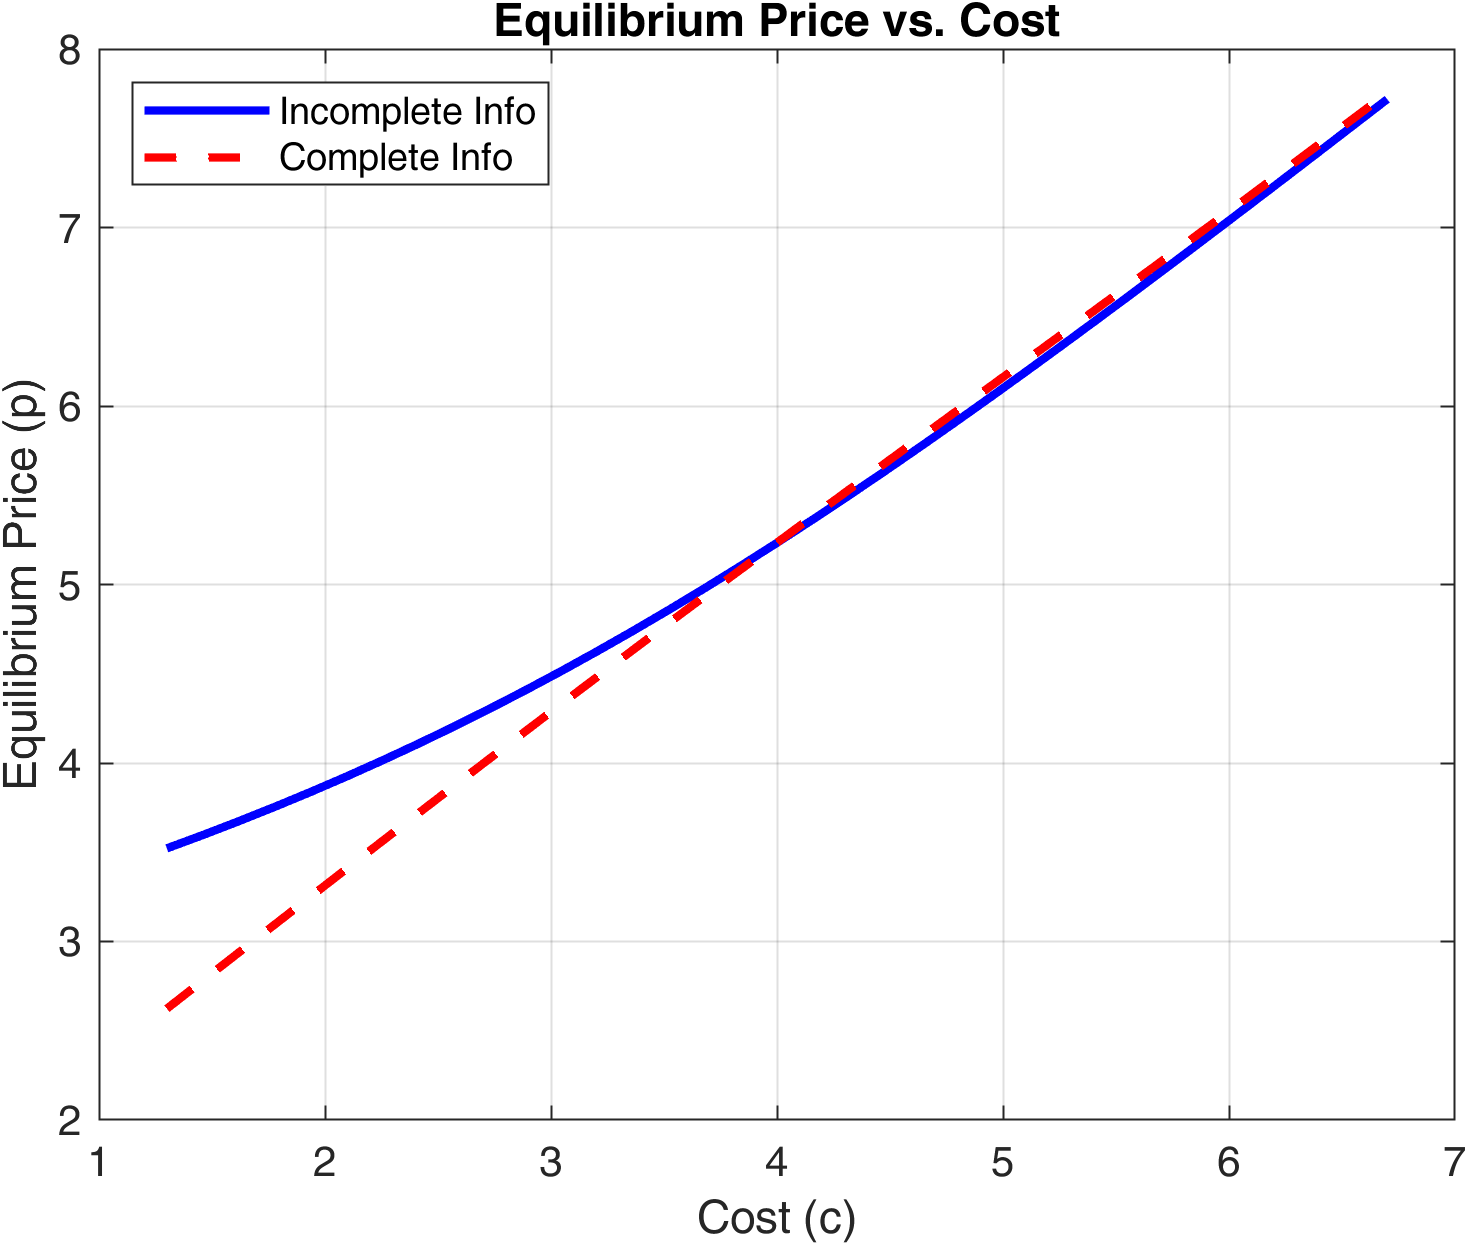
\includegraphics[scale=0.7]{../figures/simulations/model5/pricesCI_IC.png}
\end{tabular}
\end{figure}
\end{frame}

\begin{frame}{Extensions}
Possible extensions
\begin{itemize}
    \item To add search costs
    \item Allow for more than one search 
    \item Model prediction precision 
\end{itemize}
\end{frame}


\section{Appendix}


\begin{frame}{Loan estimate}\label{slide:fig_LE}    
\begin{figure}[H]
\centering{}%
\begin{tabular}{cc}
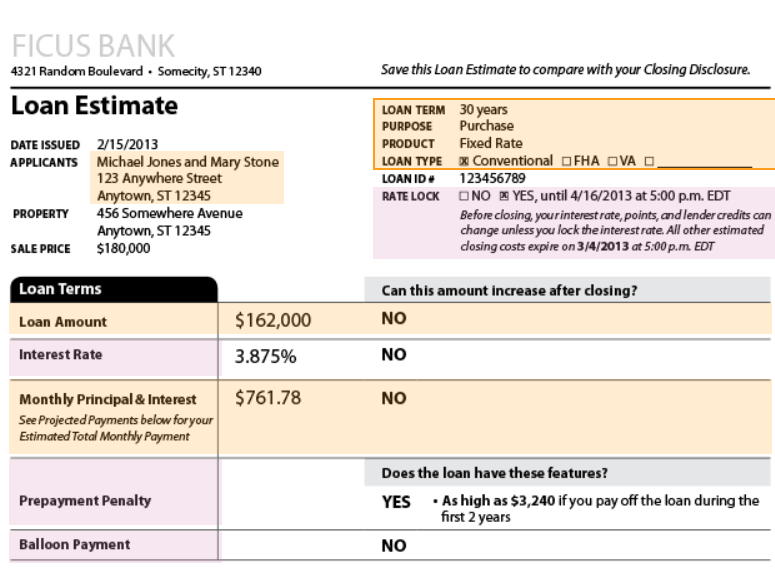
\includegraphics[scale=0.42]{../figures/docs_screenshots/Loan Estimate_cut.png}
\end{tabular}
\end{figure}
\hyperlink{slide:motivation}{\beamerbutton{Go back: Motivation}}
\end{frame}





\begin{frame}{Initial prices}\label{slide:fig_offer_certificate}    
\begin{figure}[H]
\centering{}%
\begin{tabular}{cc}
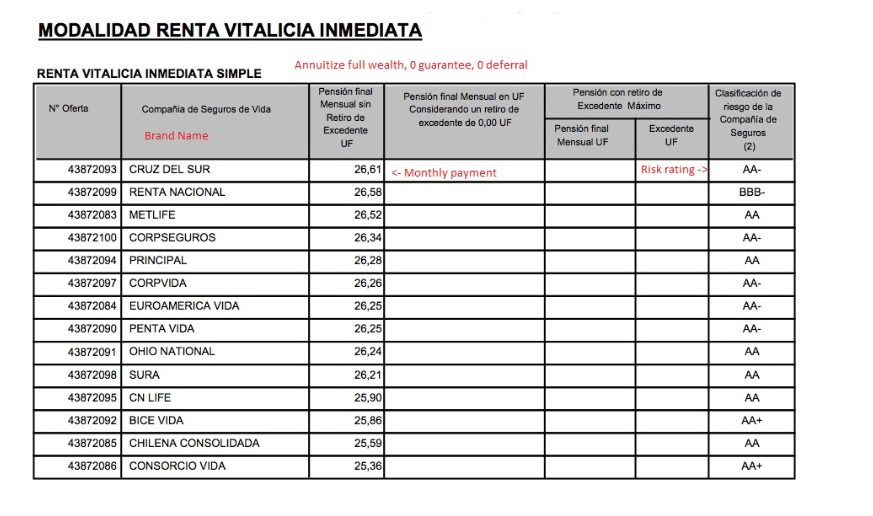
\includegraphics[scale=0.49]{../figures/docs_screenshots/annuity_offer.png}
\end{tabular}
\end{figure}
\hyperlink{slide:setting2}{\beamerbutton{Go back: Diagram}} 
\hyperlink{slide:data}{\beamerbutton{Go back: Data}}
\end{frame}


\begin{frame}{Connection model with setting}\label{slide:connection}    
\begin{itemize}
    \item Firms cost: 
    \begin{align*}
        c_{ij} =  \mathbb{E}^j_{T} \left[\sum_{t=1}^T\frac{1}{(1+r_j)^t}|x_i \right]
    \end{align*}  
    \item Firm prices: $p_j = S_i/F_{ij}$
    \item Firm profits: 
    \begin{align*}
        \pi_{ij}(F) = (p_j - c_{ij}) D_{ij} = \frac{S}{4}
    \end{align*}
\end{itemize}

\hyperlink{slide:timeline}{\beamerbutton{Go back: Timeline}}
[STILL WORK ON THIS SLIDE]
\end{frame}

\end{document}